\documentclass[11pt,a4paper]{article}
\usepackage{lac2013}
\usepackage{booktabs}
\usepackage{moreverb}
\usepackage{url}
\usepackage{graphicx}
\sloppy
\newenvironment{contentsmall}{\small}

\title{SuperCollider IDE: A Dedicated Integrated Development Environment for SuperCollider}

\author
{Jakob Leben
\\ Koper, Slovenia
\\ jakob.leben@gmail.com
\And
Tim Blechmann
\\ Vienna, Austria
\\ tim@klingt.org
}


\hyphenation{MacOS}
\hyphenation{scsynth}
\hyphenation{sclang}

\begin{document}
\maketitle


\begin{abstract}
\begin{contentsmall}
SuperCollider IDE is a new cross-platform integrated development environment for SuperCollider. It unifies user
experience across platforms and brings improvements and new features in comparison with previous coding environments,
making SuperCollider easier to begin with for new users, easier to teach for teachers, and more efficient to work with
for experienced users. We present an overview and evaluation of its features, and explain motivations from the point of
view of user experience.
\end{contentsmall}
\end{abstract}

\keywords{
\begin{contentsmall}
SuperCollider, cross-platform, edit, code, GUI
\end{contentsmall}
}

\section{Introduction}

SuperCollider \cite{rethinking-sc} is a computer music system that was originally developed by James McCartney in the
1990s for MacOS and has been ported to Linux and eventually Windows after it was open sourced in the early 2000s. It is
a modular system based on an object oriented programming language (sclang) and a separate audio synthesis server
(scsynth)\footnote{A multiprocessor-aware alternative to scsynth is supernova \cite{blechmann11icmc}}.


\subsection{History of SuperCollider and its Coding Environments}

SuperCollider is heavily influenced by Smalltalk and was originally using a similar programming model: it strongly
coupled the interpreter with the development environment. This integrated programming environment \textbf{SC.app} was
developed for Mac OS X using the Cocoa framework and therefore was not portable to other platforms. It provides both a
development environment and an implementation of GUI widgets.

When porting SuperCollider to Linux, Stefan Kersten implemented \textbf{scel}, a SuperCollider editor mode for Emacs
\cite{collision}, which had been the most feature-rich editor for SuperCollider for a long time, as it not only
supported syntax highlighting, but also some introspection, a limited form of method call assistance and support for the
old HTML-based help system.

At the moment, two other SuperCollider modes are part of the official distribution: \textbf{scvim} (for vim) or
\textbf{sced} (for gedit). Before developing the new SuperCollider IDE, one of the authors of this paper developed an
editor mode for Kate (\textbf{scate}).

Apart from that, there have been other editors or editor modes, either incomplete or not maintained anymore:
\textbf{scfront} (a Tcl/Tk based editor), \textbf{qcollider} (a Qt-based editor) and modes for the squeak Smalltalk
environment, the TextMate editor, Eclipse and probably others \cite{collision}. A python-based editor called
\textbf{PsyCollider} \cite{dos} had first been distributed with the Windows port of SuperCollider, but later removed
from
distribution, as the code was unmaintained, unstable and made obsolete when gedit and sced were ported to
Windows.

\subsection{Motivation for the New IDE}

Having multiple editors or programming environments for SuperCollider has numerous disadvantages:

\begin{itemize}
\item The user experience vastly differs among the different programming environments.
\item Each programming environment has to be maintained separately, and long-term maintenance turned out to be a
  problem. The scarce development resources are spread among different projects instead of focused on a single system.
\item No existing environment is working out of the box on every supported operating system.
\item Some environments (e.g. scvim or scel) are based on editors that are not very accessible for beginners.
\end{itemize}

In late 2011 the authors therefore decided to start the development of a new IDE dedicated to SuperCollider (not
merely an editor mode). The main motivation was to provide an IDE that would offer a unified user experience across all
supported platforms and that would be both easy to use for beginners and powerful so that experienced users don't feel the
need to switch to an advanced editor like Emacs.

Since one of the authors had also reimplemented the GUI widgets for sclang in Qt to make them cross-platform, the
choice of GUI framework for the new IDE was clear.

\section{Overview of the new IDE}

\subsection{System Architecture}

Since an IDE demands a tight integration with the target programming language, the question was
raised immediately whether the new IDE should be coupled with the language interpreter into one
process, as is the case in SC.app, or rather a separate process, as in existing editor modes.

Consideration of benefits and drawbacks of the two options brought decision in favor of
separating the IDE from the interpreter: the most important benefit of this strategy is that the
decoupling allows the IDE to survive potential crashes of the interpreter, and maintain
responsiveness and control in case running some SuperCollider code locks up in an infinite loop.

The major drawback of decoupling is increased effort for inter-process communication (IPC) with the
interpreter. However, scel has proved that a powerful set of features may be built on top of IPC,
and hence this did not outweight the benefits of decoupling.

\subsection{Graphical Interface}
\label{gui}

Thanks to the Qt GUI framework, the appearance and behavior of the GUI is largely equal across supported platforms.
Figure \ref{fig:mainwin} shows the default appearance on Ubuntu.

The IDE has a single-window design - it features a single code editing widget at the center of the main window. Tabs are
used to switch between multiple open documents. The editor widget can also be split horizontally and vertically to show
more than one document at a time.

Below the code editor, there is an area where various tool panels are displayed on request via keyboard shortcuts:
\begin{itemize}
  \item Find/Replace: a standard tool for finding and replacing text in the current document, supporting regular
expressions and backreferences in replacement
  \item Go-To-Line: a standard tool to quickly jump to a line in the current document, by line number
  \item Command Line: a tool for one-line SuperCollider expressions to be evaluated, featuring history
\end{itemize}

Along the edges of the main window, there are \emph{dock areas}, where other \emph{dockable widgets} may be placed:
\begin{itemize}
  \item Integrated help browser
  \item Document browser
  \item Language interpreter output panel
\end{itemize}

These widgets can be easily drag-and-dropped to different locations in the dock areas, either side-by-side, or stacked
on top of each other (with tabs appearing to switch among the stacked widgets). They can also be undocked and moved out
of the main window (e.g. to place them on a second screen etc.), or simply hidden.

The status bar on the bottom of the main window is used to show the state of the language interpreter and the default
synthesis server. The server status box is a compact alternative to the SuperCollider server window, showing status
information like CPU utilization, number of running synths, groups, synthdefs etc.

\begin{figure*}[]
  \centering
  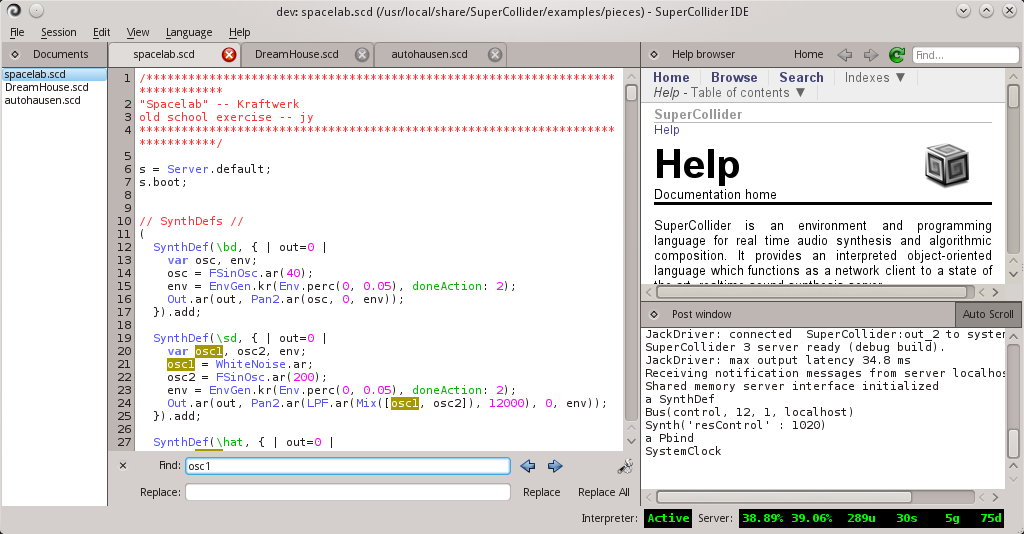
\includegraphics[width=\textwidth]{overview}
  \caption{SuperCollider IDE on Ubuntu}
  \label{fig:mainwin}
\end{figure*}

\section{Interaction}

Our guidelines in interaction design were to minimize the amount of constantly visible controls, so as not to clutter
the GUI, but to make the most used functionality quickly accessible via keyboard shortcuts, and advanced features easily
discoverable via the main menu and \emph{context menus} - i.e. menus that pop up when right-clicking (or Ctrl-clicking)
on a GUI element and offer a choice of actions relevant for that element.

To combine accessibility and discoverability the following rule is applied: as much functionality as possible is
in the main menu, and each item in any menu may be assigned a shortcut.

We distribute the IDE with a large set of default shortcuts that cover most frequently used functionality by both
SuperCollider beginners and experts, and try to adhere to shortcuts in other coding environments.

\subsection{System Control}

The language interpreter is started automatically with the IDE. Nonetheless, it can be stopped and restarted at will
via the main menu or shortcuts, which is useful if code gets stuck in an infinite loop, or the interpreter simply
crashes and stops by itself.

The audio server, on the other hand, is not started automatically, but can be quickly started using a shortcut or the
main menu. The menu includes other audio-related actions: to dump the node tree, show sound level meters and the like.
All these actions may also be accessed via the context menu associated with the audio server status box (see section
\ref{gui} about the status bar).

\subsection{Code Evaluation}
\label{code-eval}

Code evaluation is, naturally, the most valuable functionality of a SuperCollider coding environment, and making it as
practical as immaginable is of highest importance.

All existing coding environments support evaluating a line of code using a keyboard shortcut without the need to select
the line. Moreover, since SuperCollider code is often evaluated in groups of lines, there is typically support for
enclosing such groups in parenthesis, then double-clicking one of the parenthesis to select the contents in order to
evaluate them. Such groups of lines are commonly called \emph{regions}.

The SuperCollider IDE goes a step further by automatically detecting the region enclosing the text cursor, so it can be
evaluated with a shortcut without the need to select it. The evaluation behavior is intelligent: it will evaluate
either the selection (if any), or the current region (if any), or the current line - where \emph{current} means `at the
position of the cursor'.

Due to automatic region detection, large portions of code may be evaluated without selection. However, without any
visual indication, this could easily create confusion and uncertainty as to what code has been evaluated. Hence,
another very useful feature has been implemented: evaluated code is highlighted, and then the highlighting gradually
fades away. An additional benefit of highlighting is in demonstration scenarios: not only the demonstrator, but the
audience as well knows exactly what code is evaluated, and when.

\section{Code Editing}

It is our goal for SuperCollider IDE to implement code-editing assistance on the level of support
that general-purpose IDEs offer for most widely used programming languages. Namely,
we consider the crucial features: automatic indentation, syntax highlighting, automatic code completion and method call
hints.

\subsection{Automatic Indentation}
\label{auto-indentation}

The IDE automatically indents code while typing, trying to mimic the most common ways people would indent code by hand.
Automatic indentation may also be invoked explicitly for a selection of lines.

Automatic indentation is done on the basis of opening and closing brackets. When a line break is entered, the new line
is indented by one level if the previous line contains any opening brackets that are not matched with a closing bracket
on the same line. Whenever a closing bracket is typed on a subsequent line, a previous line containing the matching
opening bracket is searched for, and if the matching brackets are the first and the last ones on their lines,
respectively, the current line is made to match indentation of the line above. For example:

\begin{verbatimtab}[4]
(
p = Pseq([
	Pbind(
		\degree, Pwhite(0,5,5),
		\dur, 0.1
	),
	Pbind(\degree, Pseq([6,7]))
], inf)
)
\end{verbatimtab}

As shown above, \emph{regions} (see section \ref{code-eval}) do not contribute to indentation, as is common in
SuperCollider code.

One current issue with automatic indentation remains to be addressed: indentation of line continuations. It is common
to have one expression extend over several lines; in this case, it is typically desired to increase indentation on all
but the first line. For example:

\begin{verbatimtab}[4]
In.kr(4, 2)
	.lag(0.3)
	.linexp(0, 1, 10, 1000)
\end{verbatimtab}

This is currently not implemented yet; a solution will require enhanced grammatical analysis.

\subsection{Syntax Highlighting}
\label{syntax-highlighting}

Existing SuperCollider editor modes typically reuse generic support of their host editors for
on-the-fly syntax highlighting. SC.app, albeit the oldest and most widely used environment, only
updates highlighting on explicit request via the user interface.

Syntax highlighting in SuperCollider IDE has been implemented to update on-the-fly, and in a very
efficient manner to never interfere with code typing. Attention was paid to strictly match the
lexical rules obeyed by the SuperCollider language compiler. As a result, we have most efficient and
correct syntax highlighting for SuperCollider language to-date.

\subsection{Automatic Completion}
\label{auto-completion}

Automatic code completion (autocompletion) consists of offering the user a selection of possible
continuations of text being typed, based on context.

As a weakly-typed programming language, SuperCollider poses limitations on the possibilities of
autocompletion, compared to strongly-typed languages (e.g. C, C++). Namely, it is not always
possible to infer the type of a variable identifier, and hence the set of its methods. We have
worked in SuperCollider IDE towards offering completion as far as possible within these limitations.

Autocompletion is offered in the following cases:
\begin{itemize}
 \item Class names:

 \verb|Sin<...>|

 Since class names exclusively begin with an uppercase letter, it is straightfoward
 to complete them from the set of all classes.

 \item Method names following class names:

 \verb|Array.<...>|

 They are completed from the set of class methods of the
 readily-available class.

 \item Method names following literals and built-ins

 \verb|123.<...>|

 \verb|topEnvironment.<...>|

 They are completed from the set of instance methods of the class
 inferred from the literal or the built-in.

 \item Method names following a variable name:

 \verb|func.<...>|

 The class is not inferred, so the method is completed from the set of all methods of all classes.

\end{itemize}

Completion of methods of known classes starts immediately when the dot `.' is typed. One exception
to this is the case of methods of Integer literals: it only begins after 1 character has been
typed, or else redundant completion would be triggered on a dot in a Float literal, which proved
to be a rather annoying experience.

In other cases the list of candidates may be quite large (the set of all classes, or all methods of
all classes), hence completion only starts after 3 characters have been typed.

Although the current code base would easily support completion of built-ins (e.g.
\verb|topEnvironment|) and method names in functional notation (e.g. \verb|min(1,2)|) we have
decided to avoid that. The reason is that, formally, those cases would compete with other cases for
which we currently do not offer completion: e.g. variable names in scope. It has been argued by
one of the authors that autocompletion options may be understood (especially by novices) as the set
of all and the only allowed options in a specific context, and hence misleading when incomplete.

The completion menu is hidden if the currently typed text matches one of the options exactly. In
that case, the user's intention has likely been met, so the menu would only present an obstacle to
changing activity: evaluating code, moving to another position in code, etc. However, this has been
a point of debate, as it would be possible to automatically detect the change of activity and close
the menu.

Although different aspects of usability often demand trade-offs, we will continue to refine the
behavior so as to maximize usefulness and intuitivity of autocompletion.

As already noted, there is potential to improve the domain of autocompletion to include:
\begin{itemize}
 \item Variables in scope:

 \verb|var abcdef; abc<...>|

 \item Inferring class of Array and Event literals:

 \verb|[1,2,3].<...>|

 \verb|(freq: 321).<...>|

 \item Inferring class of variables by assignment

 \verb|x = [1,2,3]; x.<...>|

\end{itemize}

\subsection{Method Call Assistance}
\label{method-call-assistance}

Method call assistance involves displaying a list of argument names and their default values, to aid
entering expressions for arguments in a method call.

It is implemented both for receiver notation as well as functional notation. In functional notation,
an argument is prepended to denote the receiver of the message.

The assistance is invoked when a relevant opening bracket `(' is typed, or a comma `,' is typed to
separate arguments, and additionally with a keyboard shortcut when the text cursor is anywhere
within the brackets surrounding the arguments.

This assistance is subject to the same limitations as autocompletion, due to a weakly-typed
language: to disambiguate the method, its owner class must be known. However, we have found a
pragmatic solution: where the class can not be inferred, we let the user pick a class via a pop-up
menu.

Hence, the following examples will offer assistance directly:

\verb|SinOsc.ar(|

\verb|123.forBy(|

...while the following will first display a list of classes that implement the method, then offer
method call assistance once a class is selected:

\verb|min(|

\verb|x.play(|

\verb|[1,2,3].inject(|

There is one special case in SuperCollider language where the method name is not explicit, namely
an opening bracket immediately following a class name:

\verb|Synth(|

In this case, the class method `new' is implied, and SuperCollider IDE takes this into account and
offers appropriate assistance.

Once the assistance is invoked, the name of the current argument being typed is highlighted, which
is of great help when the number of arguments is large, or the expression for an argument is very
long.

Moreover, one can quickly insert and cycle through available argument names with a press of the Tab
key, in order to realize argument addressing by name, as in:

\verb|SinOsc.ar(456, add: 1, mul:|

Once assistance has been activated for a particular method call, it remains active in the
background while assistance for a nested method call is being performed: when the user
finishes typing the inner call, assistance is automatically displayed for the outer call again.

This is especially useful in case assistance is based on explicit class selection (as explained
above) - the selection is remembered during nested assistances so that method disambiguation does
not need to be repeated.

As can be seen from examples above, this assistance would also benefit from increased ability to
automatically infer classes from text. Nevertheless, the described solution via explicit class
selection will remain to be useful where the intended method is absolutely ambiguous.

\subsection{Editing Shortcuts}

Akin to powerful general-purpose development environments, SuperCollider IDE provides a set of actions that help
navigate and edit code and can be assigned arbitrary keyboard shortcuts.

Cursor movement actions include:
\begin{itemize}
  \item Jump to next or previous empty line
  \item Jump to next or previous bracket
  \item Jumping to next or previous region
\end{itemize}

Editing actions include:
\begin{itemize}
 \item Move current line up or down
 \item Copy current line up or down
 \item Comment or uncomment current line or selection
\end{itemize}

The comment/uncomment action intelligently uses either the single-line or the multi-line comment syntax,
whichever is more appropriate for the current selection.

\section{Class Library Navigation}
\label{class-lib-lookup}

Within the SuperCollider community, the border between system developers and users has always been
quite fuzzy. Furthermore, writing musical code often involves development of classes for purposes of
a specific musical task and for personal class libraries. Jumping from code that uses a class to
code that implements it is hence a frequent need.

The SuperCollider language interpreter has since the beginning featured introspection into where
each class and method is implemented, and referenced within the class library. Existing development
environments have already harnessed these capabilities to offer navigation between usage and
definition via GUI.

SuperCollider IDE attempts to exploit these capabilities in most practical ways. Handy shortcuts
will pop up a dialog that lists all methods whose name matches the text under cursor, or all methods
of the class under cursor. Pressing Return on an entry will open the file at position where the
selected method or class is implemented. The same dialog contains a search field which can be used
to search for any class or method.

An equivalent dialog is implemented also for class and method references: the listing contains
all methods that contain references to another class or method.

The shortcuts and menu actions that bring up these dialogs work just as well in the code editor,
as in any other GUI element that may contain code: the command line, the post window, and the help
browser.

Moreover, invoking help-related shortcuts within these dialogs will navigate the help browser to the
help page related to the class or method selected in the dialog. Help and class library navigation
are thus very efficiently linked.

\section{Help}

Recently, the traditional HTML-based help system has been superseded by \textbf{SCDoc}, authored by
Jonatan Liljedahl, where help documents are written in a markup language developed specifically
for this purpose, and rendered to HTML on demand. The benefits are:
\begin{itemize}
 \item Documentation is always up-to-date.
 \item Content is separate from style; consistent style can easily be applied to all documentation.
 \item Content may potentially be rendered to other formats than HTML, by implementing different
rendering components.
\end{itemize}

Interaction with SCDoc's on-demand rendering has previously only been implemented within the SuperCollider language,
using its internal GUI capabilities. The SuperCollider IDE is the first code editing environment to integrate the new
help system into its own GUI. There are two major benefits:
\begin{itemize}
 \item Tighter integration with all the GUI components.
 \item The last displayed document and the entire browsing history is preserved across class library recompilations and
interpreter restarts.
\end{itemize}

The help browser comes in form of a dockable widget (see section \ref{gui}). When the user requests help using a related
shortcut or menu action, on-demand rendering is performed via the SCDoc system, and the resulting HTML document is
displayed in the help browser.

The help system is tightly connected to many GUI components: the help shortcut will recall a relevant help document
for the text under cursor, when it is invoked within the code editor, the command line, the post window, the help
browser itself, or - as noted above - for the selected entry in the class and method implementation and reference
dialogs.

Example code in help documents may also be evaluated. Another benefit of integration with the IDE is that the shortcut
for evaluation is identical to the one in the code editor, even when customized by the user.

Moreover, the same shortcuts as in other GUI components may be used for class library lookup (see section
\ref{class-lib-lookup}).

\section{Sessions}

A \emph{session} is a snapshot of currently open documents and arrangement of GUI components that may be restored
after the IDE is restarted. The IDE allows saving a number of different sessions and quickly switching between them,
making it easy to store and recall the environment for different tasks.

\section{Configuration}

Many aspects of SuperCollider IDE can be customized, including:
\begin{itemize}
 \item behavior of automatic indentation and code evaluation
 \item colors of the editor component and syntax highlighting
 \item keyboard shortcuts
\end{itemize}

The IDE also makes easy configuration of the SuperCollider language interpreter. Class library directories to include
and exclude from compilation can be configured via the GUI, removing the need to hand-edit the interpreter's
configuration file. There is also a handy menu action to open the SuperCollider startup file.

\section{Conclusions and Ideas for Future Development}

SuperCollider IDE has successfully reached the fundamental goal of providing a cross-platform SuperCollider coding
environment. Not only has it integrated the individual strengths of previous coding environments, but it has brought
important improvements on its own. It makes SuperCollider more accessible to new users, eases education and exchange of
knowledge, as well as focuses future development work.

Immediate benefits arise from a unified experience across Linux, Mac OS X and Windows. Furthermore, sophisticated user
interface design and advanced code development assistance make it both easier to use by novices and a powerful tool for
experienced users and developers.

As described above, possibilities for improvements have been detected especially at automatic code indentation
(\ref{auto-indentation}) and completion (\ref{auto-completion}), and method call assistance
(\ref{method-call-assistance}), and are simply a matter of further work.

There are many ideas for future development:

\paragraph{SCDoc Editing Support} \hfill

Among the highest priority goals is support for syntax highlighting and editing assistance for the SCDoc markup
language. This would be a very welcome aid in writing SuperCollider documentation, and might entice conversion of
remaining old HTML-based documentation to the SCDoc format (there is a lot of unconverted documents in various Quarks).

\paragraph{Scripting IDE Behavior} \hfill

The standard SuperCollider class library includes the Document class which is used as a generic programming interface to
various coding environments. It allows for controlling the open documents and manipulating with their contents.
SuperCollider IDE does not support this interface yet, but the support for it is of high priority, including its
potential extension.

\paragraph{Code Snippets} \hfill

An alternative code editing mode could introduce code snippets as individual interactive components. This would be
an alternative for the current concept of \emph{regions} (\ref{code-eval}). The snippets would be separated at the
level of graphical interface, instead of code syntax, which could allow for instance to move them freely around a
``desk''-like area, hide and show them individually, and to evaluate their contents with a single click.

\paragraph{Visual SynthDef and Pattern Composition} \hfill

For some tasks it would be welcome to be able to compose SynthDefs and Patterns in a visual way, akin to visual
programming languages like PureData, Max, etc. Various diffuse efforts in this direction exist, mostly using the
SuperCollider language itself. Most elaborate effort is probably by Jonatan Liljedahl in his ongoing development of
algoSCore - a SuperCollider-based successor to AlgoScore \cite{algoscore}, which includes graphical composition of
SuperCollider Patterns and SynthDefs. We consider potential integration of work in this field into SuperCollider IDE as
a great benefit.

\paragraph{Integration of User-Created GUI} \hfill

GUI creation by users would also benefit from a visual composition approach, as opposed to writing SuperCollider code.
Moreover, it would be very practical if user-created GUIs could be integrated into the IDE's own GUI, as
\emph{docklets} (\ref{gui}) or similar. We believe that employing the Qt Quick technology would be a good basis for this
purpose.


\section{Acknowledgements}

The authors would like to thank the vibrant community of SuperCollider developers and users for critical evaluation of
SuperCollider IDE and many useful insights. With such a productive feedback and intensive involvement in shaping ideas,
even two lone developers never feel lonely in their efforts. SuperCollider IDE is much better because of you!

\bibliographystyle{acl}
\bibliography{sample}

\end{document}
